\documentclass[final]{beamer}
\usepackage[orientation=portrait,size=a0,
            scale=1.1         % font scale factor
           ]{beamerposter}

\geometry{
  hmargin=2.5cm, % little modification of margins
}

%
\usepackage[utf8]{inputenc}
\usepackage{tabularx}
\usepackage{booktabs}

\linespread{1.15}

\usetheme{sharelatex}


\title
[Radar-based Sentiment Analysis and Recognition] % Conference
{ % Poster title
Radar-based Sentiment Analysis and Recognition
}

\author{ % Authors
Mohamed-anas Abbouchi\inst{1}, Haider Azam\inst{2}, Mudassar Iqbal\inst{3}
}
\institute
[RF-Behavior Sentiment Recognition] % General University
{
\inst{1} Aalto University\\[0.3ex]
\inst{2} Universitat Politecnica de Catalunya\\[0.3ex]
\inst{3} Technische Universitat Braunschweig
}
\date{\today}



\begin{document}
\begin{frame}[t]
\hspace{1cm}
\begin{multicols}{3}

\section{Introduction}

\structure{Radar sensing for privacy-preserving affective computing}

Sentiment analysis has traditionally relied on text, speech, and visual data, leaving body movement as a comparatively unexplored modality despite its strong link to affective expression. Radar sensing offers a non-intrusive, privacy-preserving alternative capable of capturing subtle body movements without the limitations of cameras or wearables.

This work uses the multimodal RF-Behavior dataset to investigate radar-based sentiment recognition through three complementary approaches shown below.

\section{Dataset}

The study is built on the third campaign of the RF-Behavior dataset~\cite{zuo2025}, collected from 44 participants using 13 radars, 8 RFID tags, LoRa devices, and infrared cameras. This campaign targets six sentiment states: depression, distraction, excitement, focus, relaxation, and stress.

Radar data consists of XYZ target-position sequences over time; infrared data adds 3--6 body-part landmarks (position and orientation) sampled at 100~Hz. Prior to modeling, radar streams are time-synchronized across sensors and normalized per user to remove individual biases.

\section{Method 1: Feature-Based Classification}

Radar trajectories were segmented into 90-frame windows with a 20-frame stride, then reduced to a set of kinematic, statistical, and directional descriptors (speed, acceleration, jerk statistics, spectral measures, tortuosity, turning-angle entropy, PCA-based directionality, etc.), summarized in Table~1.

\begin{table}
\centering
\small
\begin{tabularx}{\columnwidth}{>{\bfseries}l X}
\toprule
Category & Examples \\
\midrule
Motion dynamics &
Speed, acceleration, jerk (mean, std, median, quartiles) \\

Statistical &
Speed CV, skewness, autocorrelation, spectral entropy \\

Directional &
Turn angle, tortuosity, PCA explained variance \\
\bottomrule
\end{tabularx}
\caption{Extracted trajectory features (27 per radar).}
\end{table}

With 13 radars, this yields 351 candidate features across over 600 windows. An ANOVA F-test selects the top-$k$ features per radar, and Leave-One-Subject-Out (LOSO) cross-validation guides a joint search over window size, stride, and feature count for five classifiers: SVM, LightGBM, XGBoost, CatBoost, and MLP.

\subsection{Results}

The Support Vector Machine achieved the strongest performance with a mean weighted F1-score of 0.72, outperforming the gradient-boosting models (LightGBM and XGBoost around 0.66--0.67) and CatBoost (0.62). The MLP performed comparably to the boosting methods. These results suggest that carefully engineered motion descriptors can provide strong discriminative power without requiring deep architectures.

\section{Method 2: Deep Learning with Raw Data}

This approach trains transformer encoders directly on raw radar and infrared streams from all three RF-Behavior campaigns, avoiding manual feature engineering. Radar point clouds are resampled to a data-driven optimal rate of 18.7~FPS, balancing temporal frame count against spatial point density per frame.

The architecture (Figure~1) uses a Point Cloud Encoder (a BERT-style self-attention block, without positional encoding for radar) to condense spatial points into a single per-frame vector, followed by a Temporal Encoder (a LLaMA-style causal decoder with rotary embeddings) that condenses the frame sequence into a single recording-level embedding. For infrared data, an optional convolutional downsampling block can further compress the temporal axis.

\vskip1ex
\begin{figure}
\centering
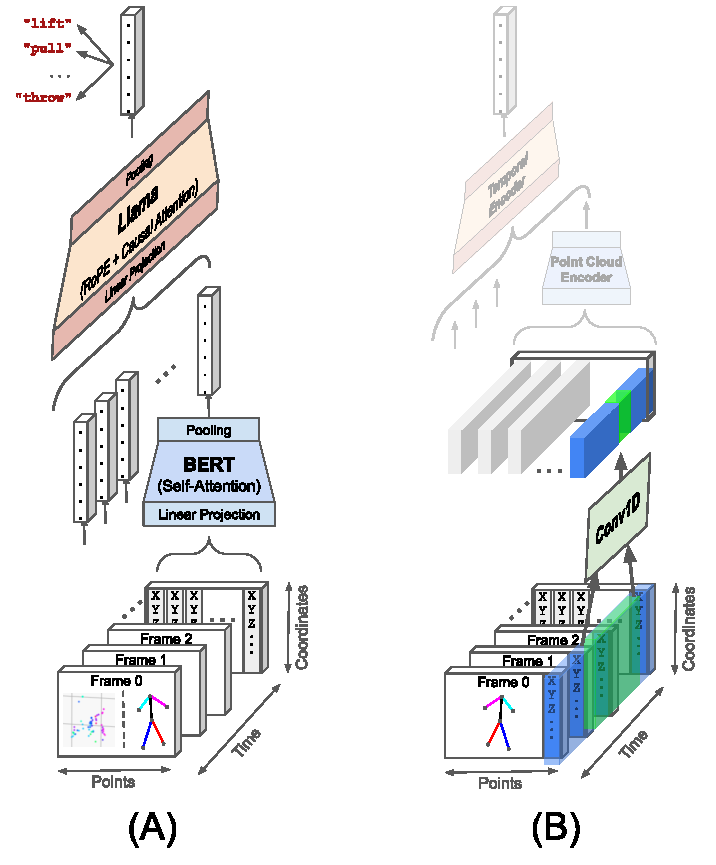
\includegraphics[width=0.99\columnwidth]{mudassar_model.pdf}
\caption{Dual Transformer pipeline}
\end{figure}
\vskip2ex

Both supervised classification (cross-entropy loss, user-level split) and unsupervised contrastive learning (NT-Xent loss, class-level split) were evaluated, along with a hyperparameter search over convolutional depth, transformer depth, attention heads, embedding size, and pooling strategy.

\subsection{Results}

\begin{table}[!t]
\centering
\small
\setlength{\tabcolsep}{3pt}
\begin{tabularx}{\columnwidth}{l c X r c c}
\toprule
\textbf{Campaign} &
\textbf{Classes} &
\textbf{Type} &
\textbf{Params} &
\textbf{Test-F1} &
\textbf{Models} \\
\midrule
C1       & 21 & Radar    & 1,311,125 & 94.41\% & 12 \\
C1       & 21 & IR &   526,869 & 96.56\% & 25 \\
C2       & 10 & Radar    &   106,826 & 91.97\% & 23 \\
C2       & 10 & IR & 1,541,850 & 98.12\% & 29 \\
C3       &  6 & Radar    & 1,349,766 & 46.12\% & 30 \\
C3       &  6 & IR &   243,798 & 56.16\% & 56 \\
\midrule
C1+C2    & 31 & Radar    &   120,895 & 89.51\% &  6 \\
C1+C2    & 31 & IR &   195,375 & 91.52\% &  5 \\
C1+C2+C3 & 37 & Radar    &   268,453 & 83.74\% &  5 \\
C1+C2+C3 & 37 & IR &   165,269 & 78.29\% &  7 \\
\bottomrule
\end{tabularx}
\caption{Results for supervised classification models.}
\label{tab:supervised_results}
\end{table}

\begin{table}
\centering
\small
\setlength{\tabcolsep}{3pt}
\begin{tabularx}{\columnwidth}{l c X r c c}
\toprule
\textbf{Campaign} &
\textbf{Split} &
\textbf{Type} &
\textbf{Params} &
\textbf{Test-F1} &
\textbf{Models} \\
\midrule
C1       & 17-2-2 & Radar    & 254,144 & 93.03\% & 6 \\
C1       & 17-2-2 & IR & 142,016 & 96.68\% & 7 \\
C2       & 6-2-2  & Radar    & 93,440  & 77.51\% & 14 \\
C2       & 6-2-2  & IR & 923,280 & 93.48\% & 31 \\
\midrule
C1+C2    & 23-4-4 & Radar    & 175,776 & 90.31\% & 7 \\
C1+C2    & 23-4-4 & IR & 282,176 & 88.13\% & 7 \\
C1+C2+C3 & 25-6-6 & Radar    & 817,472 & 79.20\% & 7 \\
C1+C2+C3 & 25-6-6 & IR & 85,184  & 75.41\% & 7 \\
\bottomrule
\end{tabularx}
\caption{Results for one-shot unsupervised classification.
(Split: \# train-valid-test behavior classes)}
\label{tab:unsupervised_results}
\end{table}

\section{Method 3: Neural Interpolation \& Classification}

Because the 13 radar sensors report at irregular, asynchronous timestamps, this method jointly learns to interpolate the sensor streams onto a common timeline and classify the resulting sequence into one of the six emotion classes.

Sequences are built per user/emotion by concatenating all 13 radars' XYZ values (39 features), with 10--30\% of each sequence randomly withheld as interpolation targets. Three interpolation/classification models are compared against a cubic-spline-plus-ridge baseline: a Neural Controlled Differential Equation (NCDE) model, a 1D U-Net, and a Temporal Convolutional Network (TCN). The NCDE integrates a differentiable Hermite-spline control signal to obtain a continuously updating hidden state, in contrast to the discrete updates of RNNs.

\vskip1ex
\begin{figure}
\centering
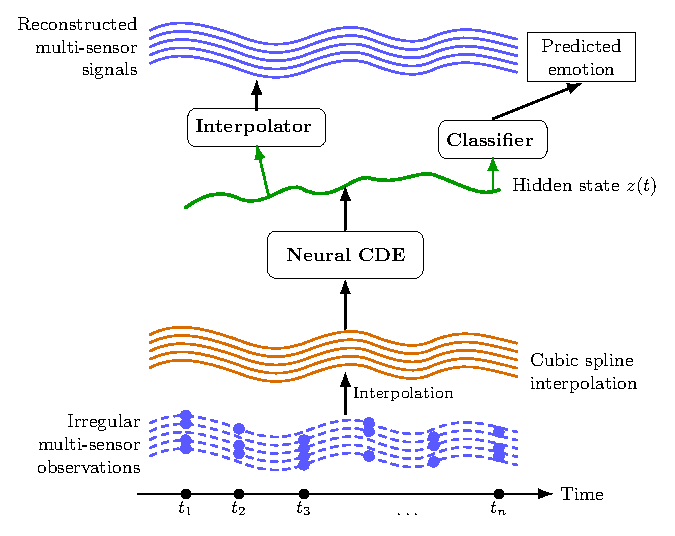
\includegraphics[width=0.99\columnwidth]{haider_workflow.pdf}
\caption{Workflow of the NCDE-based interpolation and classification pipeline: the sparse input sequence is converted to a continuous Hermite-spline control signal, integrated to obtain hidden states, then decoded for value reconstruction and classified for emotion probabilities.}
\end{figure}
\vskip2ex

\subsection{Results}
\begin{table}
\centering
\small
\setlength{\tabcolsep}{8pt}
\begin{tabular}{l c c c}
\toprule
\textbf{Method} &
\textbf{MSE} &
\textbf{Loss} &
\textbf{Accuracy (\%)} \\
\midrule
Baseline & 0.0962 & -- & -- \\
NCDE & 0.0999 & 3.617 & 44.44 \\
U-Net & 0.0995 & 1.792 & 16.67 \\
TCN & 0.0992 & 1.744 & 25.00 \\
U-Net + Baseline & 0.0962 & 1.792 & 16.67 \\
TCN + Baseline & 0.1039 & 1.650 & 33.33 \\
\bottomrule
\end{tabular}
\caption{Interpolation and classification results.}
\end{table}
\section{Summary and Conclusions}

Across all three methodologies, radar sensing shows clear promise for privacy-preserving sentiment recognition, though performance on subtle emotional states remains behind that on simpler, more repetitive behaviors, and behind infrared-based approaches. Feature-based SVM classification proved the most robust and data-efficient approach on the emotion classes studied. Deep learning on raw data generalizes well to unseen behaviors in the unsupervised setting but degrades on fine-grained emotion recognition. Joint interpolation-classification remains constrained by limited data.

Promising future directions include multimodal fusion of radar with infrared, data augmentation (sensor dropout, noise injection, geometric transforms), architectures tailored to point-cloud and irregular-time-series structure, and aligning learned sensor representations with text encoders to enable zero-shot recognition of new behaviors.

\subsection{References}

\begin{thebibliography}{99}

\bibitem{zuo2025} S.~Zuo, Y.~Song, S.~Golipoor, Y.~Liu, X.~Ma, S.~Sigg, RF-Behavior: A multimodal radio-frequency dataset for human behavior and emotion analysis, 2025.

\bibitem{chen2020} T.~Chen, S.~Kornblith, M.~Norouzi, G.~Hinton, A simple framework for contrastive learning of visual representations, \textit{ICML}, 2020.

\bibitem{radford2021} A.~Radford et al., Learning transferable visual models from natural language supervision, \textit{ICML}, 2021.

\bibitem{vaswani2017} A.~Vaswani et al., Attention is all you need, \textit{NeurIPS}, 2017.

\bibitem{kidger2020} P.~Kidger, J.~Morrill, J.~Foster, T.~Lyons, Neural controlled differential equations for irregular time series, \textit{NeurIPS}, 2020.

\end{thebibliography}

\end{multicols}

\end{frame}
\end{document}